
\begin {figure}
 \centering
  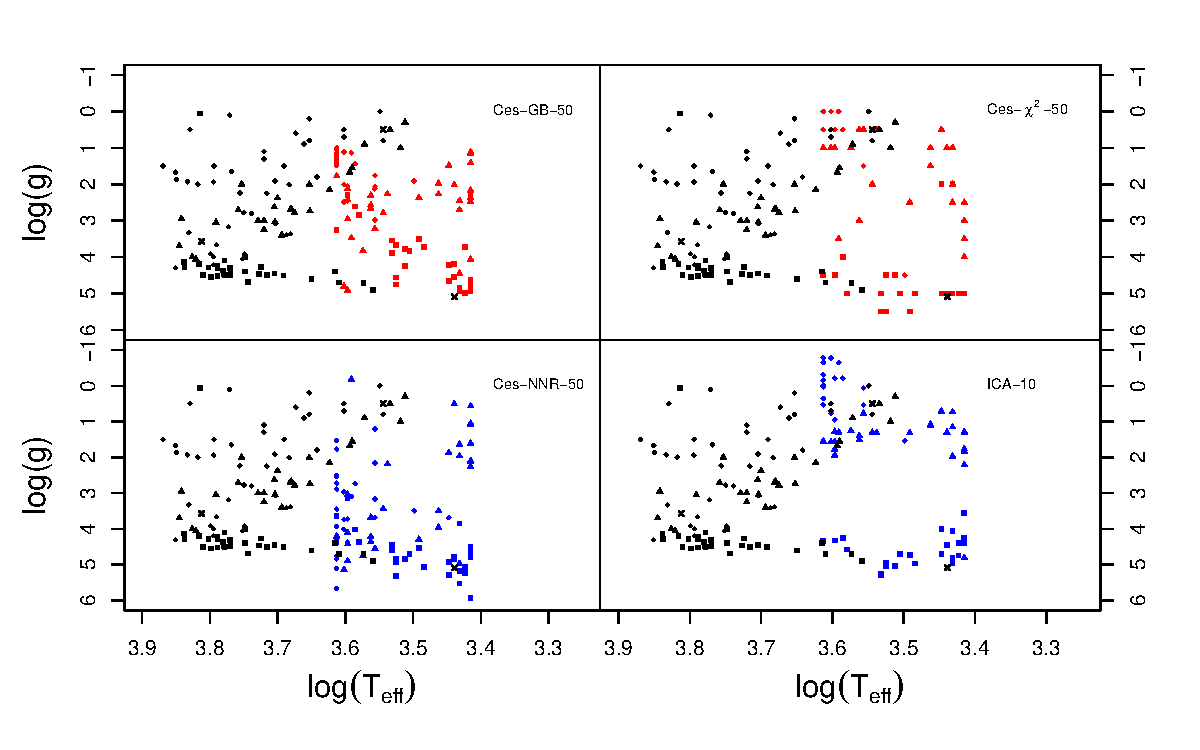
\includegraphics[width=11cm]{figs/irtf-Cesseti.pdf}
  \caption{}
 \label{fig:irtf-ces}
\end {figure}
 
 
For metallicities, we again find that the only feature space that results in reasonable results is based on ICA projections and SNR=10. Comparison of the correlation coefficients of the various regression results with the literature values shows no significant difference between the GA-based features and those taken from \cite{cesetti}. Therefore, neither set is competitive with the ICA projections. In Fig. \ref{irtf-cs-met} we show the results of the regression technique that results in the highest correlation with the literature values (RF-50).  

\begin {figure}
\centering
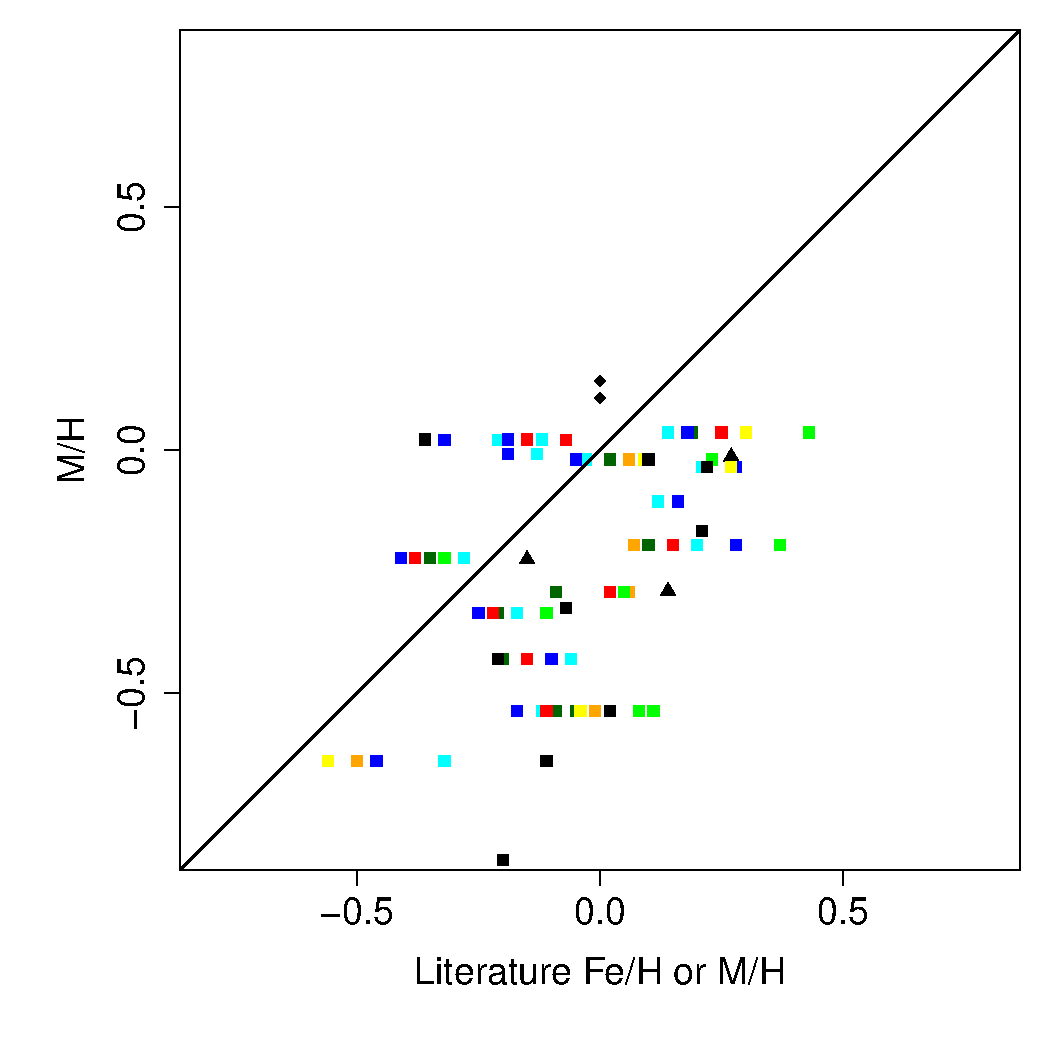
\includegraphics[width=11cm]{figs/M-CES.pdf.pdf}
\caption{}
\label{fig:irtf-ces-met}
\end {figure}
